\chapter{Foundations}
\label{chap:foundations}

This chapter introduces the theoretical concepts required for the remainder of this thesis. Section~\ref{sec:foundations_graphs} formalizes causal graphs and defines binary causal questions as reachability problems. Section~\ref{sec:foundations_astar} presents heuristic search and the $A^*$ algorithm. Section~\ref{sec:foundations_repr} introduces transformer-based embedding models and their use for graph search. Section~\ref{sec:foundations_matryoshka} presents Matryoshka Representation Learning. Finally, Section~\ref{sec:foundations_activation} introduces the non-linear activation functions used within the training objective.

\section{Causal Graphs and Binary Causal Questions}
\label{sec:foundations_graphs}

Causal knowledge graphs provide a structured representation of causal relationships that would otherwise remain implicit in unstructured text~\cite{heindorf:2020,li:2020}. They can be modeled as directed graphs \(G=(V,E)\), where nodes represent concepts or events and directed edges encode causal relations between them. This structure enables algorithmic reasoning over causal dependencies. Figure~\ref{fig:causal_types} illustrates three common causal structures, namely a causal chain, a common cause, and a common effect. Given two concepts $A$ and $B$, let $a,b \in V$ denote their corresponding graph nodes. The binary question ``Does $A$ cause $B$?'' then reduces to determining whether a directed path exists from $a$ to $b$~\cite{bluebaum:2024}\looseness=-1:
\[
\exists \; (a = v_0, v_1, \dots, v_k = b)
\text{ such that }
\forall i \in \{0,\dots,k-1\} \; (v_i, v_{i+1}) \in E.
\]
If such a path exists, the query is answered positively under this graph-based formulation. If no path can be found, either no causal relation is encoded in the graph or the available knowledge is incomplete. This formulation enables the application of classical graph traversal algorithms for causal reasoning.

\begin{figure}[t]
    \centering
    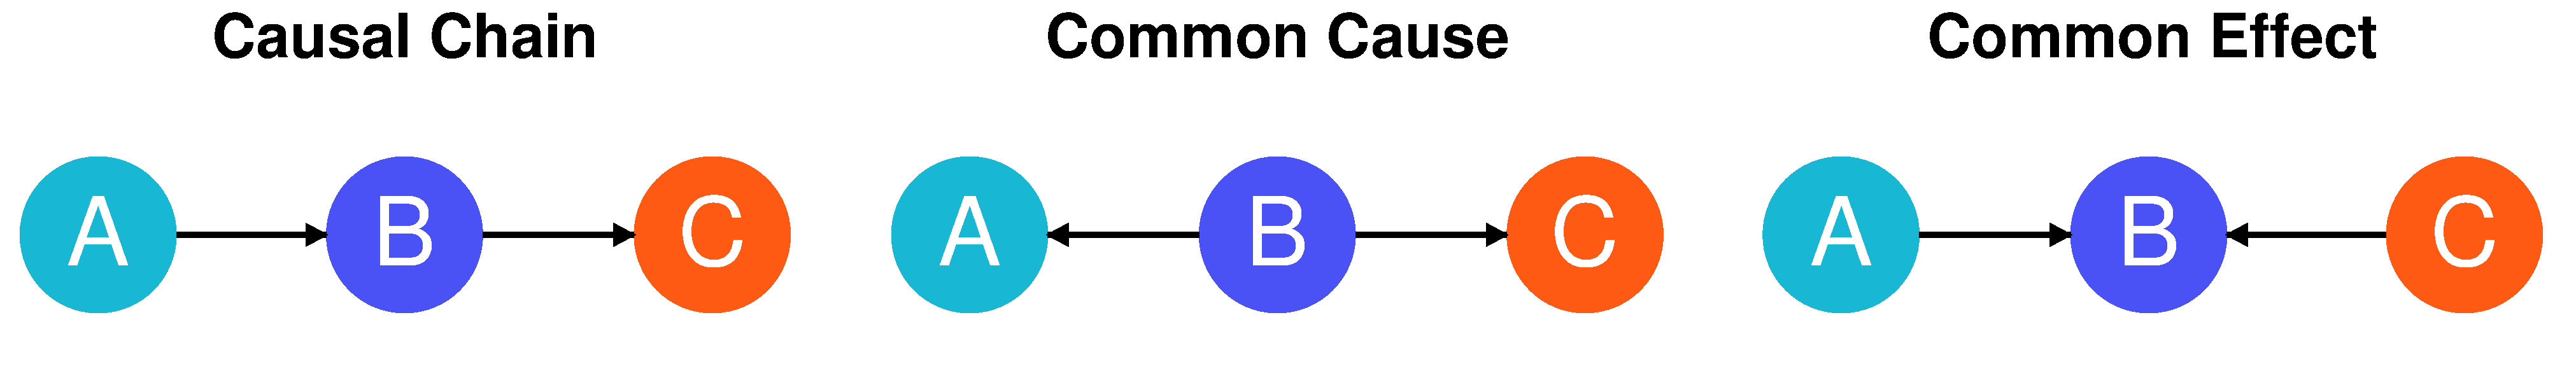
\includegraphics[width=\linewidth]{figures/causal_relation_patterns.pdf}
    \caption{Three common causal structures in directed graphs, showing a causal chain, a common cause, and a common effect.}
    \label{fig:causal_types}
\end{figure}

\section{Heuristic Search and the \texorpdfstring{$A^*$}{A*} Algorithm}
\label{sec:foundations_astar}

Graph traversal can be performed using uninformed or informed search algorithms. Uninformed search methods, such as BFS, explore the graph without guidance and guarantee completeness~\cite{cormen:2022}. However, their computational cost can be high in large graphs with significant branching factors. Heuristic search algorithms incorporate problem-specific information to guide exploration. The $A^*$ algorithm is an informed best-first search strategy~\cite{hart:1968} that selects nodes based on an evaluation function
\[
f(n) = g(n) + h(n),
\]
where $g(n)$ denotes the cost of the path from the start node to node $n$, $h(n)$ is a heuristic estimate of the remaining cost from $n$ to the target node, and $f(n)$ represents the estimated total cost of a solution path passing through $n$. At each step, $A^*$ expands the node with the smallest $f(n)$ value. The properties of $A^*$ depend on the quality of the heuristic function. Two important properties are consistency and admissibility~\cite{hart:1968}. A heuristic is \emph{consistent} if, for every node $n$ and each successor $s$, it satisfies
\[
h(n) \leq c(n,s) + h(s),
\]
where $c(n,s)$ is the cost of transitioning from $n$ to $s$. Consistency implies that $f$-values are non-decreasing along every path. Consequently, once a node has been expanded, it does not need to be reopened. A weaker condition is \emph{admissibility}, which requires that the heuristic never overestimates the true remaining cost:
\[
h(n) \leq d(n),
\]
where $d(n)$ denotes the optimal cost from node $n$ to the goal. If the heuristic is admissible, $A^*$ is guaranteed to find an optimal path when closed nodes can be reopened after a cheaper path is discovered. Without consistency, such re-expansions may be necessary.

\section{Representation Learning for Graph Search}
\label{sec:foundations_repr}

Modern natural language processing systems commonly represent textual concepts as dense vector embeddings. Transformer-based architectures form the basis of many state-of-the-art embedding models. A transformer encoder maps an input text sequence to contextualized token representations through self-attention mechanisms~\cite{vaswani:2017}. Sentence transformer models aggregate contextualized token representations into fixed-dimensional embeddings, forming a geometric space in which semantically related concepts tend to be located closer together~\cite{reimers:2019}. In graph search settings, such geometric structure can be used to guide exploration toward promising regions of the graph. Given two embeddings $\mathbf{x}, \mathbf{y} \in \mathbb{R}^d$, similarity or distance can be measured using metrics such as cosine similarity or Euclidean distance. Cosine similarity~\cite{manning:2008} is defined as
\[
\text{cosine}(\mathbf{x}, \mathbf{y}) =
\frac{\mathbf{x} \cdot \mathbf{y}}{\|\mathbf{x}\|\|\mathbf{y}\|}.
\]
It lies in the interval $[-1,1]$. In this work, cosine distance is computed as
\[
d_{\text{cos}}(\mathbf{x}, \mathbf{y}) = 1 - \text{cosine}(\mathbf{x}, \mathbf{y}),
\]
which lies in $[0,2]$. If either vector has zero norm, the cosine distance is set to $1.0$ to avoid division by zero. The second distance measure considered in this work is Euclidean distance~\cite{manning:2008}, defined as
\[
d_{\text{Euc}}(\mathbf{x}, \mathbf{y}) =
\|\mathbf{x} - \mathbf{y}\|_2.
\]
In this thesis, an embedding-guided variant of $A^*$ search is employed. Let $\phi(v)$ denote the embedding of node $v$. The cost of traversing an edge from node $n$ to a successor $s$ is defined as the distance between their embeddings, while $g(n)$ is the sum of these edge costs along the path from the start node to $n$. The heuristic $h(n)$ is the embedding distance from $n$ to the target node $b$. When Euclidean distance is used, consistency follows directly from the triangle inequality. For every successor $s$ of node $n$,
\[
h(n)
=
\lVert \phi(n)-\phi(b)\rVert_2
\leq
\lVert \phi(n)-\phi(s)\rVert_2
+
\lVert \phi(s)-\phi(b)\rVert_2
=
c(n,s)+h(s).
\]
The heuristic therefore satisfies the consistency condition of $A^*$. In contrast, cosine distance does not generally satisfy the standard triangle inequality and therefore does not guarantee heuristic consistency~\cite{schubert:2021}.

\section{Matryoshka Representation Learning}
\label{sec:foundations_matryoshka}

Standard embedding models are typically trained to produce representations with a fixed dimensionality. If such an embedding is truncated to a smaller number of dimensions, there is generally no guarantee that the reduced vector retains meaningful structure.
Matryoshka Representation Learning~\cite{kusupati:2022} addresses this limitation by optimizing multiple prefix subspaces of an embedding to remain informative. Let $\mathbf{e} \in \mathbb{R}^d$ denote a learned embedding vector with full dimensionality $d$. Instead of optimizing only the full representation, the model is trained such that several nested prefix dimensionalities
\[
m_1 < m_2 < \dots < m_k = d
\]
preserve useful structural information. For each dimensionality $m_i$, the corresponding truncated embedding is defined as
\[
\mathbf{e}_{m_i} = \mathbf{e}_{1:m_i},
\]
where $\mathbf{e}_{1:m_i}$ denotes the prefix consisting of the first $m_i$ components of the full embedding vector. The training objective is applied at multiple prefix dimensionalities, encouraging each truncated embedding to retain task-relevant information. This promotes an ordered representation in which earlier dimensions capture broadly useful features, while later dimensions add finer-grained information and additional capacity~\cite{kusupati:2022}. This property enables a trade-off between representational capacity and computational efficiency. In applications such as graph search, reducing embedding dimensionality can lower the cost of distance computations while preserving sufficient information for effective heuristic guidance. However, overly small prefixes may discard too much information and degrade the quality of the heuristic.

\section{Activation Functions}
\label{sec:foundations_activation}

Neural networks rely on non-linear activation functions to model complex relationships between inputs and outputs. Without non-linearities, stacked linear transformations would collapse into a single linear mapping, severely limiting representational power. One widely used activation function is the Rectified Linear Unit (ReLU)~\cite{nair:2010}, defined as
\[
\text{ReLU}(x) = \max(0, x).
\]
ReLU maps negative inputs to zero while preserving positive inputs. Its simple piecewise-linear form allows for efficient computation. Another commonly used activation function is the Gaussian Error Linear Unit (GELU)~\cite{hendrycks:2016}, defined as
\[
\text{GELU}(x) = x \cdot \Phi(x),
\]
where $\Phi(x)$ denotes the cumulative distribution function of the standard normal distribution.
\begin{figure}[htbp]
    \centering
    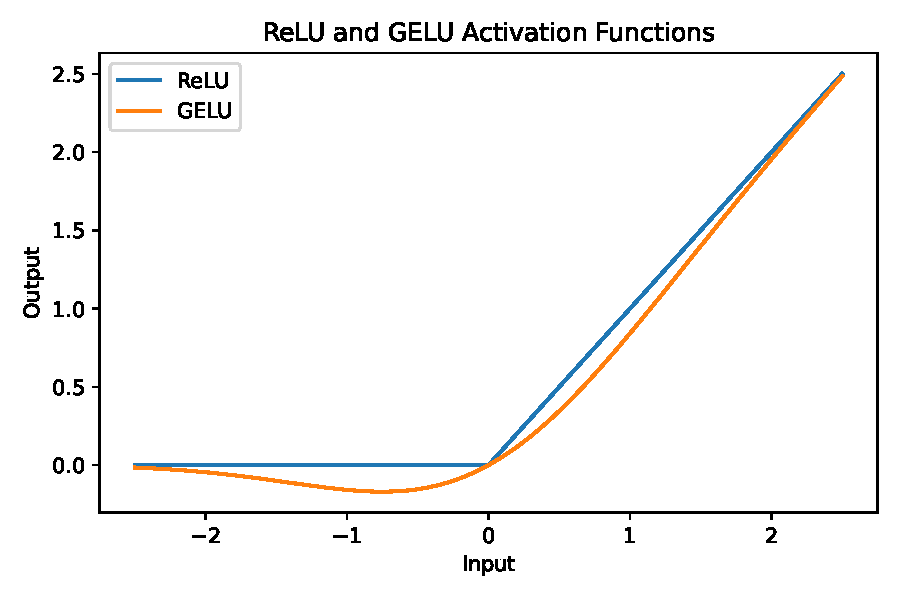
\includegraphics[width=1\linewidth]{figures/relu_gelu}
    \caption{Comparison of ReLU and GELU activation functions.}
    \label{fig:relu_gelu}
\end{figure}
In practical implementations, GELU is often approximated using a tanh-based formulation~\cite{hendrycks:2016}:
\[
\text{GELU}(x) \approx 0.5x \left(1 + \tanh\left(\sqrt{\frac{2}{\pi}} \left(x + 0.044715x^3\right)\right)\right),
\]
which provides a computationally efficient approximation while preserving the smooth gating behavior of the original function. Unlike ReLU, which applies a hard threshold at zero, GELU provides a smooth activation that weights inputs according to their magnitude. Figure~\ref{fig:relu_gelu} illustrates this difference. In this thesis, ReLU and GELU are evaluated as non-linear transformations within the training objective. Their different shapes determine how score differences are transformed and how strongly they contribute to the loss, thereby shaping the learned embedding space used by the $A^*$ heuristic.